\chapter{Pseudorandomness}\label{Pseudorandomness}

\paragraph{Reading:} Katz-Lindell Section 3.3, Boneh-Shoup Chapter 3

The nature of randomness has troubled philosophers, scientists,
statisticians and laypeople for many years.\footnote{Even lawyers
  grapple with this question, with a recent example being the debate of
  whether fantasy football is a game of chance or of skill.} Over the
years people have given different answers to the question of what does
it mean for data to be random, and what is the nature of probability.
The movements of the planets initially looked random and arbitrary, but
then the early astronomers managed to find \emph{order} and make some
\emph{predictions} on them. Similarly we have made great advances in
predicting the weather, and probably will continue to do so. So, while
these days it seems as if the event of whether or not it will rain a
week from today is \emph{random}, we could imagine that in with time we
will be able to predict the weather further into the future. Even the
canonical notion of a random experiment -tossing a coin - turns out that
it \href{http://statweb.stanford.edu/~susan/papers/headswithJ.pdf}{might
not be as random as you'd think}, with about a 51\% chance that the
second toss will have the same result as the first one. (Though
\href{https://www.stat.berkeley.edu/~aldous/Real-World/coin_tosses.html}{see
also this experiment}.) It is conceivable that at some point someone
would discover some function \(F\) that given the first 100 coin tosses
by any given person can predict the value of the 101\(^{th}\).\footnote{In
  fact such a function must exist in some sense since in the entire
  history of the world, presumably no sequence of \(100\) fair coin
  tosses has ever repeated.} In all these examples, the physics
underlying the event, whether it's the planets' movement, the weather,
or coin tosses, did not change but only our powers to predict them. So
to a large extent, \emph{randomness is a function of the observer}, or
in other words

\begin{quote}
\emph{If a quantity is hard to compute, it might as well be random.}
\end{quote}

Much of cryptography is about trying to make this intuition more formal,
and harnessing it to build secure systems. The basic object we want is
the following:

\hypertarget{prgdefconcrete}{}
\begin{definition}[Pseudorandom generator (concrete)] \label[definition]{prgdefconcrete}

A function \(G:{\{0,1\}}^n\rightarrow{\{0,1\}}^\ell\) is a
\((T,\epsilon)\) \emph{pseudorandom generator} if
\(G(U_n) \approx_{T,\epsilon} U_\ell\) where \(U_t\) denotes the uniform
distribution on \({\{0,1\}}^t\).

\end{definition}

That is, \(G\) is a \((T,\epsilon)\) pseudorandom generators if no
circuit of at most \(T\) gates can distinguish with bias better than
\(\epsilon\) between the output of \(G\) (on a random input) and a
uniformly random string of the same length.

As we did for the case of encryption, we will typically use
\emph{asymptotic terms} to describe cryptographic pseudorandom
generator. We say that \(G\) is simply a pseudorandom generator if it is
\((p(n),1/p(n))\)-pseudorandom generator for every polynomial
\(p(\cdot)\). In other words, we define pseudorandom generators as
follows

\hypertarget{prgdef}{}
\begin{definition}[Pseudorandom generator] \label[definition]{prgdef}

Let \(G:\{0,1\}^* \rightarrow \{0,1\}^*\) be some function computable in
polynomial time. We say that \(G\) is a \emph{pseudorandom generator}
with length function \(\ell:\N \rightarrow \N\) (where \(\ell(n)>n\))if

\begin{itemize}
\item
  For every \(x\in \{0,1\}^*\), \(|G(x)| = \ell(|x|)\).
\item
  For every polynomial \(p(\cdot)\) and sufficiently large \(n\), the
  function \(G_n\) (the restriction of \(G\) to inputs of length \(n\))
  is a \((p(n),\tfrac{1}{p(n)})\) pseudorandom generator.
\end{itemize}

\end{definition}

Equivalently, \(G\) as above is a pseudorandom generator if the two
distributions \(G(U_n)\) and \(U_{\ell(n)}\) are \emph{computationally
indistinguishable}.

\begin{pause} \label[pause]{This-definition-as-is-oft}

This definition (as is often the case in cryptography) is a bit long, so
you want to take your time parsing it. In particular you should verify
that you understand why the condition \eqref{prgdefeq} is the same as
saying that for every polynomial \(p:\N \rightarrow \N\), if \(n\) is
sufficiently large, then for every circuit \(D\) of at most \(T\) gates
(or equivalently, for every straightline program \(D\) of at most \(T\)
lines):
\[\left| \Pr[D(G(U_n))=1] - \Pr[ D(U_\ell)=1] \right| < \tfrac{1}{p(n)} \label{prgdefeq}\]

\end{pause}

Note that the requirement that \(\ell>n\) is crucial to make this notion
non-trivial, as for \(\ell=n\) the function \(G(x)=x\) clearly satisfies
that \(G(U_n)\) is identical to (and hence in particular
indistinguishable from) the distribution \(U_n\). (Make sure that you
understand this last statement!) However, for \(\ell>n\) this is no
longer trivial at all, and in particular if we didn't restrict the
running time of \(Eve\) then no such pseudo-random generator would
exist:

\hypertarget{breakprglem}{}
\begin{lemma} \label[lemma]{breakprglem}

Suppose that \(G:{\{0,1\}}^n\rightarrow{\{0,1\}}^{n+1}\). Then there
exists an (inefficient) algorithm
\(Eve:{\{0,1\}}^{n+1}\rightarrow{\{0,1\}}\) such that
\({\mathbb{E}}[ Eve(G(U_n)) ]=1\) but
\({\mathbb{E}}[ Eve(U_{n+1})] \leq 1/2\).

\end{lemma}

\begin{proof} \label[proof]{On-input-yinn-consider-th}

On input \(y\in{\{0,1\}}^{n+1}\), consider the algorithm \(Eve\) that
goes over all possible \(x\in{\{0,1\}}^n\) and will output \(1\) if and
only if \(y=G(x)\) for some \(x\). Clearly
\({\mathbb{E}}[ Eve(G(U_n)) ] =1\). However, the set
\(S =\{ G(x) : x\in {\{0,1\}}^n \}\) on which Eve outputs \(1\) has size
at most \(2^n\), and hence a random \(y{\leftarrow_{\tiny R}} U_{n+1}\)
will fall in \(S\) with probability at most \(1/2\).

\end{proof}

It is not hard to show that if \(P=\ensuremath{\mathit{NP}}\) then the
above algorithm Eve can be made efficient. In particular, at the moment
we do not know how to \emph{prove} the existence of pseudorandom
generators. Nevertheless they are widely believed to exist and hence we
make the following conjecture:

\begin{quote}
\textbf{Conjecture (The PRG conjecture):} For every \(n\), there exists
a pseudorandom generator \(G\) mapping \(n\) bits to \(n+1\)
bits.\footnote{The name ``The PRG conjecture'' is non-standard. In the
  literature this is known as the conjecture of existence of
  pseudorandom generators. This is a weaker form of ``The Optimal PRG
  Conjecture'' presented in my \href{https://goo.gl/G7bU4M}{intro to
  theoretical CS lecture notes} since the PRG conjecture only posits the
  existence of pseudorandom generators with arbitrary polynomial blowup,
  as opposed to an exponential blowup posited in the optimal PRF
  conjecture.}
\end{quote}

As was the case for the cipher conjecture, and any other conjecture,
there are two natural questions regarding the PRG conjecture: why should
we believe it and why should we care. Fortunately, the answer to the
first question is simple: it is known that the cipher conjecture
\emph{implies} the PRG conjecture, and hence if we believe the former we
should believe the latter. (The proof is highly non-trivial and we may
not get to see it in this course.) As for the second question, we will
see that the PRG conjecture implies a great number of useful
cryptographic tools, including the cipher conjecture (i.e., the two
conjectures are in fact equivalent). We start by showing that once we
can get to an output that is one bit longer than the input, we can in
fact obtain any number of bits.

\hypertarget{lengthextendprgthm}{}
\begin{theorem}[Length Extension for PRG's] \label[theorem]{lengthextendprgthm}

Suppose that the PRG conjecture is true. Then for every polynomial
\(t(n)\), there exists a pseudorandom generator mapping \(n\) bits to
\(t(n)\) bits.

\end{theorem}


\begin{figure}
\centering
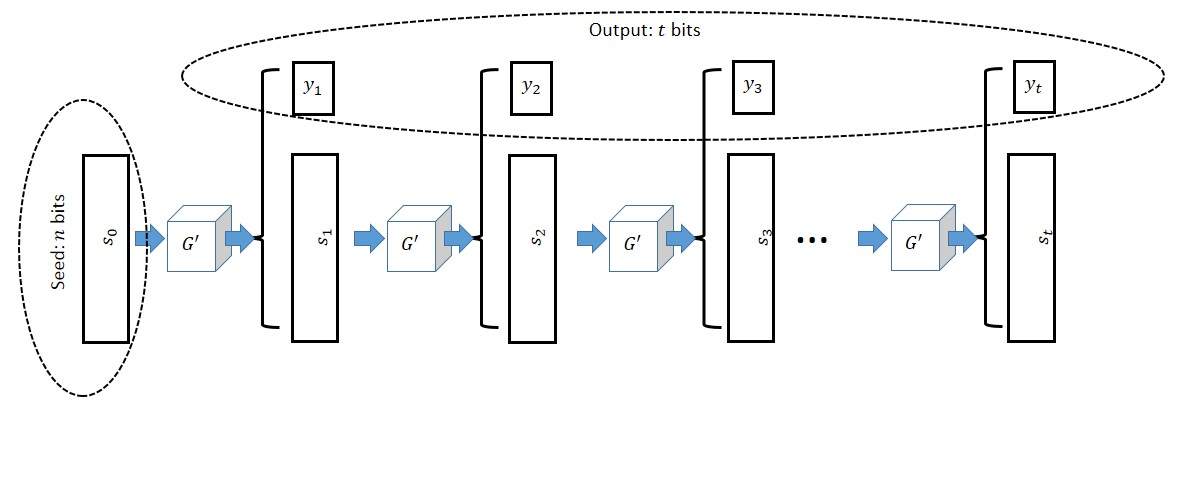
\includegraphics[width=\textwidth, height=0.25\paperheight, keepaspectratio]{../figure/length-extension-prg.jpg}
\caption{Length extension for pseudorandom generators}
\label{lengthextendprgfig}
\end{figure}

\begin{proof} \label[proof]{The-proof-of-this-theorem}

The proof of this theorem is very similar to the length extension
theorem for ciphers, and in fact this theorem can be used to give an
alternative proof for the former theorem.

The construction is illustrated in \cref{lengthextendprgfig}. We are
given a pseudorandom generator \(G'\) mapping \(n\) bits into \(n+1\)
bits and need to construct a pseudorandom generator \(G\) mapping \(n\)
bits to \(t=t(n)\) bits for some polynomial \(t(\cdot)\). The idea is
that we maintain a state of \(n\) bits, which are originally our input
seed\footnote{Because we use a small input to grow a large pseudorandom
  string, the input to a pseudorandom generator is often known as its
  \emph{seed}.} \(s_0\), and at the \(i^{th}\) step we use \(G'\) to map
\(s_{i-1}\) to the \(n+1\)-long bit string \((s_i,y_i)\), output \(y_i\)
and keep \(s_i\) as our new state. To prove the security of this
construction we need to show that the distribution
\(G(U_n) = (y_1,\ldots,y_t)\) is computationally indistinguishable from
the uniform distribution \(U_t\). As usual, we will use the hybrid
argument. For \(i\in\{0,\ldots,t\}\) we define \(H_i\) to be the
distribution where the first \(i\) bits chosen at uniform, whereas the
last \(t-i\) bits are computed as above. Namely, we choose \(s_i\) at
random in \(\{0,1\}^n\) and continue the computation of
\(y_{i+1},\ldots,y_t\) from the state \(s_i\). Clearly \(H_0=G(U_n)\)
and \(H_t=U_t\) and hence by the triangle inequality it suffices to
prove that \(H_i \approx H_{i+1}\) for all \(i\in\{0,\ldots,t-1\}\). We
illustrate these two hybrids in \cref{lengthextendhybridfig}.


\begin{figure}
\centering
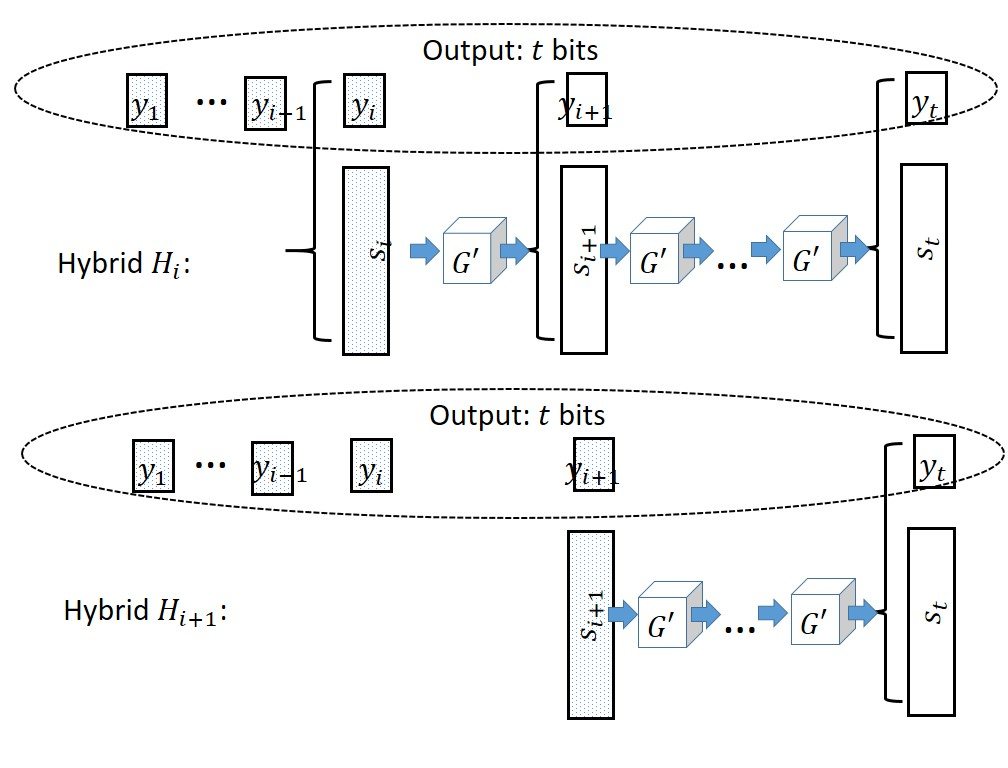
\includegraphics[width=\textwidth, height=0.25\paperheight, keepaspectratio]{../figure/length-extension-prg-hybrid.jpg}
\caption{Hybrids \(H_i\) and \(H_{i+1}\)--- dotted boxes refer to values
that are chosen independently and uniformly at random}
\label{lengthextendhybridfig}
\end{figure}

Now suppose otherwise, that there exists some adversary \(Eve\) such
that \(\left| \E[Eve(H_i)] - \E[Eve(H_{i+1})] \right| \geq \epsilon\)
for some non-negligible \(\epsilon\). We will build from \(Eve\) an
adversary \(Eve'\) breaking the security of the pseudorandom generator
\(G'\) (see \cref{reductionlengthextendfig}).


\begin{figure}
\centering
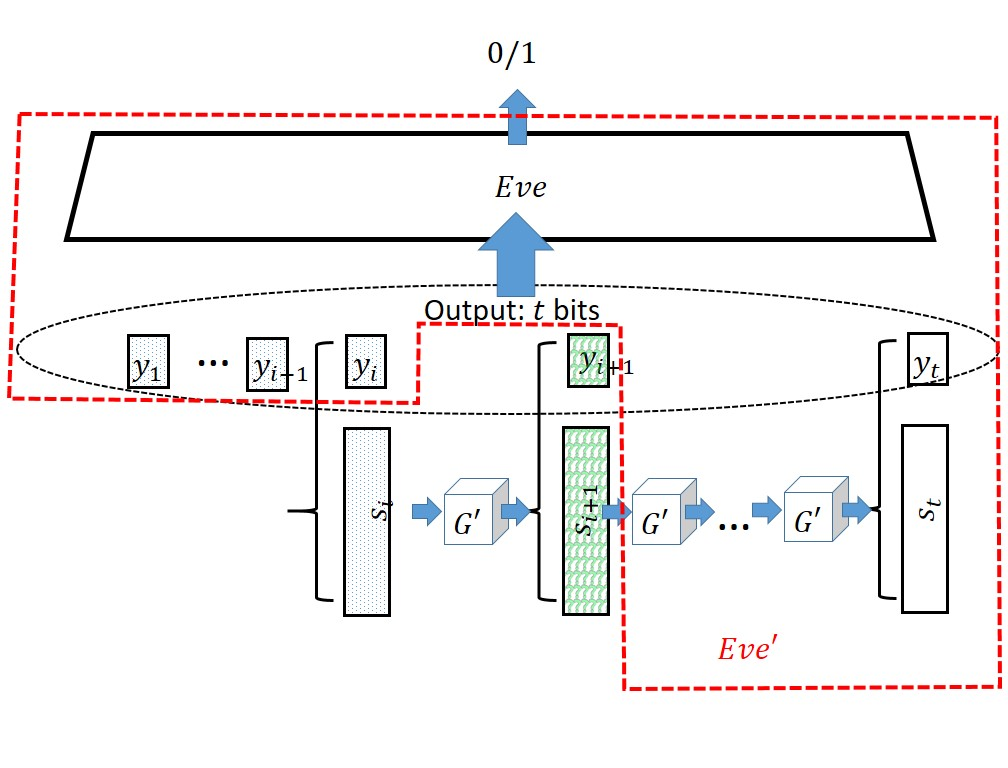
\includegraphics[width=\textwidth, height=0.25\paperheight, keepaspectratio]{../figure/length-extension-prg-adversary.jpg}
\caption{Building an adversary \(Eve'\) for \(G'\) from an adversary
\(Eve\) distinguishing \(H_i\) and \(H_{i+1}\). The boxes marked with
questions marks are those that are random or pseudorandom depending on
whether we are in \(H_i\) or \(H_{i+1}\). Everything inside the dashed
red lines is simulated by \(Eve'\) that gets as input the \(n+1\)-bit
string \((s_{i+1},y_{i+1})\).}
\label{reductionlengthextendfig}
\end{figure}

On input of string \(y\) of length \(n+1\), \(Eve'\) will interpret
\(y\) as \((s_{i+1},y_{i+1})\), choose \(y_1,\ldots,y_i\) randomly and
compute \(y_{i+2},\ldots,y_t\) as in our pseudorandom generator's
construction. \(Eve'\) will then feed \((y_1,\ldots,y_t)\) to \(Eve\)
and output whatever \(Eve\) does. Clearly, \(Eve'\) is efficient if
\(Eve\) is. Moreover, one can see that if \(y\) was random then \(Eve'\)
is feeding \(Eve\) with an input distributed according to \(H_{i+1}\)
while if \(y\) was of the form \(G(s)\) for a random \(s\) then \(Eve'\)
will feed \(Eve\) with an input distributed according to \(H_i\). Hence
we get that \(| \E[ Eve'(G'(U_n))] - \E[Eve'(U_{n+1})] | \geq \epsilon\)
contradicting the security of \(G'\).

\end{proof}

The proof of \cref{lengthextendprgthm} is indicative of many practical
constructions of pseudorandom generators. Many operating systems keep
track of an initial \emph{seed} of randomness, and supply a system call
\texttt{rand} such that every call to \texttt{rand} applies a
pseudorandom generator \(G'\) to the current seed, uses part of the
output to update the seed, and returns the remainder to the caller.

\hypertarget{alternativelengthextendrem}{}
\begin{remark}[Unpredictablity and indistinguishability- an alternative approach for proving the length extension theorem] \label[remark]{alternativelengthextendrem}

The notion that being random is the same as being ``unpredictable'' can
be formalized as follows. One can show that a random variable \(X\) over
\(\{0,1\}^n\) is pseudorandom if and only if every efficient algorithm
\(A\) succeeds in the following experiment with probability at most
\(1/2+negl(n)\): \(A\) is given \(i\) chosen at random in
\(\{0,\ldots,n-1\}\) and \(x_1,\ldots,x_i\) where \((x_1,\ldots,x_n)\)
is drawn from \(X\) and wins if it outputs \(x_{i+1}\). It is a good
optional exercise to prove this, and to use that to give an alternative
proof of the length extension theorem.

\end{remark}

\section{Stream ciphers}\label{Stream-ciphers}

We now show a connection between our two notions:

\hypertarget{PRGandcipherthm}{}
\begin{theorem}[PRG conjecture implies  Cipher conjectures] \label[theorem]{PRGandcipherthm}

If the PRG conjecture is true then so is the cipher conjecture.

\end{theorem}

It turns out that the converse direction is also true, and hence these
two conjectures are \emph{equivalent}, though we will probably not show
the (quite non-trivial) proof of this fact in this course. (We might
show some weaker version of this harder direction.)

\begin{proof} \label[proof]{The-construction-is-actua}

The construction is actually quite simple, recall that the \emph{one
time pad} is a perfectly secure cipher but its only problem was that to
encrypt an \(n+1\) long message it needed an \(n+1\) long bit key. Now
using a pseudorandom generator, we can map an \(n\)-bit long key into an
\(n+1\)-bit long string that looks random enough that we could use it as
a key for the one-time pad. That is, our cipher will look as follows:

\[
E_k(m) = G(k) \oplus m
\]

and

\[
D_k(c) = G(k) \oplus c
\]

Just like in the one time pad,
\(D_k(E_k(m)) = G(k) \oplus G(k) \oplus m = m\). Moreover, the
encryption and decryption algorithms are clearly efficient and so the
only thing that's left is to prove security or that for every pair
\(m,m'\) of plaintexts, \(E_{U_n}(m) \approx E_{U_n}(m')\). We show this
by proving the following claim:

\textbf{Claim:} For every \(m\in{\{0,1\}}^{n+1}\),
\(E_{U_n}(m) \approx U_{n+1} \oplus m\).

The claim implies the security of the scheme, since it means that
\(E_{U_n}(m)\) is indistinguishable from the one-time-pad encryption of
\(m\), which is identically distributed to the one-time pad encryption
of \(m'\) which (by another application of the claim) is
indistinguishable from \(E_{U_n}(m')\) and so the theorem follows from
the triangle inequality. Thus all that's left is to prove the claim:

\textbf{Proof of claim:} Suppose that there was an efficient adversary
\(Eve'\) such that

\[
\left| {\mathbb{E}}[ Eve'(G(U_n)\oplus m)] - {\mathbb{E}}[ Eve'(U_{n+1}\oplus m) ] \right| \geq \epsilon
\]

for some non-negligible \(\epsilon=\epsilon(n)>0\). Then the adversary
\(Eve\) defined as \(Eve(y) = Eve'(y\oplus m)\) would be also efficient
and would break the security of the PRG with non-negligible success.
This concludes the proof of the claim and hence the theorem.

\end{proof}

If the PRG outputs \(t(n)\) bits instead of \(n+1\) then we
automatically get an encryption scheme with \(t(n)\) long message
length. In fact, in practice if we use the length extension for PRG's,
we don't need to decide on the length of messages in advance. Every time
we need to encrypt another bit (or another block) \(m_i\) of the
message, we run the basic PRG to update our state and obtain some new
randomness \(y_i\) that we can XOR with the message and output. Such
constructions are known as \emph{stream ciphers} in the literature. In
much of the practical literature the name \emph{stream cipher} is used
both for the pseudorandom generator itself, as well as for the
encryption scheme that is obtained by combining it with the one-time
pad.

\hypertarget{cointossingphonerm}{}
\begin{remark}[Using pseudorandom generators for coin tossing over the phone] \label[remark]{cointossingphonerm}

The following is a cute application of pseudorandom generators. Alice
and Bob want to toss a fair coin over the phone. They use a pseudorandom
generator \(G:\{0,1\}^b\rightarrow\{0,1\}^{3n}\).

\begin{itemize}
\tightlist
\item
  Alice will send \(z\leftarrow_R\{0,1\}^{3n}\) to Bob\\
\item
  Bob picks \(s\leftarrow_R\{0,1\}^n\) and with probability \(1/2\)
  sends \(G(s)\) (case I) and with probability \(1/2\) sends
  \(G(s)\oplus z\) (case II).\\
\item
  Alice then picks a random \(b\leftarrow_R\{0,1\}\) and sends it to
  Bob.\\
\item
  Bob reveals what he sent in the previous stage and if it was case I,
  their output is \(b\), and if it was case II, their output is \(1-b\).
\end{itemize}

It can be shown that (assuming the protocol is completed) the output is
a random coin, which neither Alice or Bob can control or predict with
more than negligible advantage over half. (Trying to formalize this and
prove it is an excellent exercise.)

\end{remark}

\section{What do pseudorandom generators actually look
like?}\label{What-do-pseudorandom-gene}

So far we have made the conjectures that objects such as ciphers and
pseudorandom generators \emph{exist}, without giving any hint as to how
they would actually look like. (Though we have examples such as the
Caesar cipher, Vignere, and Enigma of what secure ciphers \emph{don't}
look like.) As mentioned above, we do not know how to \emph{prove} that
any particular function is a pseudorandom generator. However, there are
quite simple \emph{candidates} (i.e., functions that are conjectured to
be secure pseudorandom generators), though care must be taken in
constructing them. We now consider candidates for functions that maps
\(n\) bits to \(n+1\) bits (or more generally \(n+c\) for some constant
\(c\) ) and look at least somewhat ``randomish''. As these constructions
are typically used as a basic component for obtaining a longer length
PRG via the length extension theorem (\cref{lengthextendprgthm}), we
will think of these pseudorandom generators as mapping a string
\(s\in\{0,1\}^n\) representing the current state into a string
\(s’\in\{0,1\}^n\) representing the new state as well as a string
\(b\in\{0,1\}^c\) representing the current output. See also Section 6.1
in Katz-Lindell and (for greater depth) Sections 3.6-3.9 in the
Boneh-Shoup book.

\subsection{Attempt 0: The counter
generator}\label{Attempt--The-counter-gene}

Just to get started, let's show an example of an obviously bogus
pseudorandom generator. We define the ``counter pseudorandom generator''
\(G:\{0,1\}^n \rightarrow \{0,1\}^{n+1}\) as follows. \(G(s)=(s',b)\)
where \(s' = s + 1 \mod 2^n\) (treating \(s\) and \(s'\) as numbers in
\(\{0,\ldots,2^n-1\}\)) and \(b\) is the least significant digit of
\(s'\). It's a great exercise to work out why this is \emph{not} a
secure pseudorandom generator.

\begin{pause} \label[pause]{You-should-really-pause-h}

You should really pause here and make sure you see why the ``counter
pseudorandom generator'' is not a secure pseudorandom generator. Show
that this is true even if we replace the least significant digit by the
\(k\)-th digit for every \(0 \leq k < n\).

\end{pause}

\subsection{Attempt 1: The linear checksum / linear feedback shift
register (LFSR)}\label{Attempt--The-linear-check}

LFSR can be thought of as the ``mother'' (or maybe more like the sick
great-uncle) of all psuedorandom generators. One of the simplest ways to
generate a ``randomish'' extra digit given an \(n\) digit number is to
use a \emph{checksum} - some linear combination of the digits, with a
canonical example being the
\href{https://en.wikipedia.org/wiki/Cyclic_redundancy_check}{cyclic
redundancy check} or CRC.\footnote{CRC are often used to generate a
  ``control digit'' to detect mistypes of credit card or social security
  card number. This has very different goals than its use for
  pseudorandom generators, though there are some common intuitions
  behind the two usages.} This motivates the notion of a \emph{linear
feedback shift register generator} (LFSR): if the current state is
\(s\in\{0,1\}^n\) then the output is \(f(s)\) where \(f\) is a linear
function (modulo 2) and the new state is obtained by right shifting the
previous state and putting \(f(s)\) at the leftmost location. That is,
\(s'_1 = f(s)\) and \(s'_i = s_{i-1}\) for \(i\in\{2,\ldots,n\}\).

LFSR's have several good properties- if the function \(f(\cdot)\) is
chosen properly then they can have very long \emph{periods} (i.e., it
can take an exponential number of steps until the state repeats itself),
though that also holds for the simple ``counter'' generator we saw
above. They also have the property that every individual bit is equal to
\(0\) or \(1\) with probability exactly half (the counter generator also
shares this property).

A more interesting property is that (if the function is selected
properly) every two coordinates are independent from one another. That
is, there is some super-polynomial function \(t(n)\) (in fact \(t(n)\)
can be exponential in \(n\)) such that if
\(\ell \neq \ell' \in \{0,\ldots, t(n) \}\), then if we look at the two
random variables corresponding to the \(\ell\)-th and \(\ell'\)-th
output of the generator (where randomness is the initial state) then
they are distributed like two independent random coins. (This is
non-trivial to show, and depends on the choice of \(f\) - it is a
challenging but useful exercise to work this out.) The counter generator
fails badly at this condition: the least significant bits between two
consecutive states always flip.

There is a more general notion of a \emph{linear generator} where the
new state can be any invertible linear transformation of the previous
state. That is, we interpret the state \(s\) as an element of \(\Z_q^t\)
for some integers \(q,t\),\footnote{A ring is a set of elements where
  addition and multiplication are defined and obey the natural rules of
  associativity and commutativity (though without necessarily having a
  multiplicative inverse for every element). For every integer \(q\) we
  define \(\Z_q\) (known as the \emph{ring of integers modulo \(q\)}) to
  be the set \(\{0,\ldots,q-1\}\) where addition and multiplication is
  done modulo \(q\).} and let \(s’=F(s)\) and the output \(b=G(s)\)
where \(F:\Z_q^t\rightarrow\Z_q^t\) and \(G:\Z_q^t\rightarrow\Z_q\) are
invertible linear transformations (modulo \(q\)). This includes as a
special case the \emph{linear congruential generator} where \(t=1\) and
the map \(F(s)\) corresponds to taking \(as \pmod{q}\) where \(a\) is
number co-prime to \(q\).

All these generators are unfortunately insecure due to the great bane of
cryptography- the \emph{Gaussian elimination algorithm} which students
typically encounter in any linear algebra class.\footnote{Despite the
  name, the algorithm goes at least as far back as the Chinese
  \emph{Jiuzhang Suanshu} manuscript, circa 150 B.C.}

\hypertarget{gaussianelimthm}{}
\begin{theorem}[The unfortunate theorem for cryptography] \label[theorem]{gaussianelimthm}

There is a polynomial time algorithm to solve \(m\) linear equations in
\(n\) variables (or to certify no solution exists) over any ring.

\end{theorem}

Despite its seeming simplicity and ubiquity, Gaussian elimination (and
some generalizations and related algorithms such as Euclid's extended
g.c.d algorithm and the LLL lattice reduction algorithm) has been used
time and again to break candidate cryptographic constructions. In
particular, if we look at the first \(n\) outputs of a linear generator
\(b_1,\ldots,b_n\) then we can write linear equations in the unknown
initial state of the form \(f_1(s)=b_1,\ldots,f_n(s)=b_n\) where the
\(f_i\)'s are known linear functions. Either those functions are
\emph{linearly independent}, in which case we can solve the equations to
get the unique solution for the original state \(s\) and from which
point we can predict all outputs of the generator, or they are
dependent, which means that we can predict some of the outputs even
without recovering the original state. Either way the generator is
\(*\sharp !\)'ed (where \(* \sharp !\) refers to whatever verb you
prefer to use when your system is broken). See also this
\href{http://alumni.cs.ucr.edu/~jsun/random-number.pdf}{1977 paper} of
James Reed.

\hypertarget{nocryptoprgs}{}
\begin{remark}[Non-cryptographic PRGs] \label[remark]{nocryptoprgs}

The above means that it is a bad idea to use a linear checksum as a
pseudorandom generator in a cryptographic application, and in fact in
any adversarial setting (e.g., one shouldn't hope that an attacker would
not be able to reverse engineer the algorithm\footnote{That number is
  obtained by applying an algorithm of \href{https://goo.gl/SL8ahM}{Hans
  Peter Luhn} which applies a simple map to each digit of the card and
  then sums them up modulo 10.} that computes the control digit of a
credit card number). However, that does not mean that there are no
legitimate cases where linear generators can be used . In a setting
where the application is not adversarial and you have an ability to
\emph{test} if the generator is actually successful, it might be
reasonable to use such insecure non-cryptographic generators. They tend
to be more efficient (though often not by much) and hence are often the
default option in many programming environments such as the
\texttt{C rand()} command. (In fact, the real bottleneck in using
cryptographic pseudorandom generators is often the generation of
\emph{entropy} for their seed, as discussed in the previous lecture, and
not their actual running time.)

\end{remark}

\subsection{From insecurity to
security}\label{From-insecurity-to-securi}

It is often the case that we want to ``fix'' a broken cryptographic
primitive, such as a pseudorandom generator, to make it secure. At the
moment this is still more of an art than a science, but there are some
principles that cryptographers have used to try to make this more
principled. The main intuition is that there are certain properties of
computational problems that make them more amenable to algorithms (i.e.,
``easier'') and when we want to make the problems useful for
cryptography (i.e., ``hard'') we often seek variants that don't possess
these properties. The following table illustrates some examples of such
properties. (These are not formal statements, but rather is intended to
give some intuition )

\begin{longtable}[]{@{}ll@{}}
\toprule
Easy & Hard\tabularnewline
\midrule
\endhead
Continuous & Discrete\tabularnewline
Convex & Non-convex\tabularnewline
Linear & Non-linear (degree \(\geq 2\))\tabularnewline
Noiseless & Noisy\tabularnewline
Local & Global\tabularnewline
Shallow & Deep\tabularnewline
Low degree & High degree\tabularnewline
\bottomrule
\end{longtable}

Many cryptographic constructions can be thought of as trying to
transform an easy problem into a hard one by moving from the left to the
right column of this table.

The \textbf{discrete logarithm problem} is the discrete version of the
continuous real logarithm problem. The \textbf{learning with errors
problem} can be thought of as the noisy version of the linear equations
problem (or the discrete version of least squares minimization). When
constructing \textbf{block ciphers} we often have \emph{mixing}
transformation to ensure that the dependency structure between different
bits is \emph{global}, \emph{S-boxes} to ensure \emph{non-linearity},
and many \emph{rounds} to ensure \emph{deep} structure and \emph{large
algebraic degree}.

This also works in the other direction. Many algorithmic and machine
learning advances work by embedding a discrete problem in a continuous
convex one. Some attacks on cryptographic objects can be thought of as
trying to recover some of the structure (e.g., by embedding modular
arithmetic in the real line or ``linearizing'' non linear equations).

\subsection{Attempt 2: Linear Congruential Generators with dropped
bits}\label{Attempt--Linear-Congruent}

One approach that is widely used in implementations of pseudorandom
generators is to take a linear generator such as the linear congruential
generators described above, and use for the output a ``chopped'' version
of the linear function and drop some of the least significant bits. The
operation of dropping these bits is non-linear and hence the attack
above does not immediately apply. Nevertheless, it turns out this attack
can be generalized to handle this case, and hence even with dropped bits
Linear Congruential Generators are completely insecure and should be
used (if at all) only in applications such as simulations where there is
no adversary. Section 3.7.1 in the Boneh-Shoup book describes one attack
against such generators that uses the notion of \emph{lattice
algorithms} that we will encounter later in this course in very
different contexts.

\section{Successful examples}\label{Successful-examples}

Let's now describe some \emph{successful} (at least per current
knowledge) pseudorandom generators:

\subsection{Case Study 1: Subset Sum
Generator}\label{Case-Study--Subset-Sum-Ge}

Here is an extremely simple generator that is yet still secure\footnote{Actually
  modern computers will be able to break this generator via brute force,
  but if the length and number of the constants were doubled (or perhaps
  quadrupled) this should be sufficiently secure, though longer to write
  down.} as far as we know.

\begin{code}
# seed is a list of 40 zero/one  values
# output is a 48 bit integer
def subset_sum_gen(seed):
  modulo = 0x1000000
  constants = [  
     0x3D6EA1, 0x1E2795, 0xC802C6, 0xBF742A, 0x45FF31,  
     0x53A9D4, 0x927F9F, 0x70E09D, 0x56F00A, 0x78B494,  
     0x9122E7, 0xAFB10C, 0x18C2C8, 0x8FF050, 0x0239A3,  
     0x02E4E0, 0x779B76, 0x1C4FC2, 0x7C5150, 0x81E05E,  
     0x154647, 0xB80E68, 0xA042E5, 0xE20269, 0xD3B7F3,  
     0xCC5FB9, 0x0BFC55, 0x847AE0, 0x8CFDF8, 0xE304B7,
     0x869ACE, 0xB4CDAB, 0xC8E31F, 0x00EDC7, 0xC50541,  
     0x0D6DDD, 0x695A2F, 0xA81062, 0x0123CA, 0xC6C5C3 ]

  # return the modular sum of the constants
  # corresponding to ones in the seed
  return reduce(lambda x,y: (x+y) % modulo,
                map(lambda a,b: a*b, constants,seed))
\end{code}

The seed to this generator is an array \texttt{seed} of 40 bits, with 40
hardwired constants each 48 bits long (these constants were generated at
random, but are fixed once and for all, and are not kept secret and
hence are not considered part of the secret random seed). The output is
simply
\[\sum_{i=1}^{40} \texttt{seed}[i]\texttt{constants}[i] \pmod{2^{48}}\]
and hence expands the \(40\) bit input into a \(48\) bit output.

This generator is loosely motivated by the ``subset sum'' computational
problem, which is NP hard. However, since NP hardness is a \emph{worst
case} notion of complexity, it does not imply security for pseudorandom
generators, which requires hardness of an \emph{average case} variant.
To get some intuition for its security, we can work out why (given that
it seems to be linear) we cannot break it by simply using Gaussian
elimination.

\begin{pause} \label[pause]{This-is-an-excellent-poin}

This is an excellent point for you to stop and try to answer this
question on your own.

\end{pause}

Given the known constants and known output, figuring out the set of
potential seeds can be thought of as solving a \emph{single} equation in
40 variables. However, this equation is clearly overdetermined, and will
have a solution regardless of whether the observed value is indeed an
output of the generator, or it is chosen uniformly at random.

More concretely, we can use linear-equation solving to compute (given
the known constants \(c_1,\ldots,c_{40} \in \Z_{2^{48}}\) and the output
\(y \in \Z_{2^{48}}\)) the linear subspace \(V\) of all vectors
\((s_1,\ldots,s_{40}) \in (\Z_{2^{48}})^{40}\) such that
\(\sum s_i c_i = y \pmod{2^{48}}\). But, regardless of whether \(y\) was
generated at random from \(\Z_{2^{48}}\), or \(y\) was generated as an
output of the generator, the subspace \(V\) will always have the same
dimension (specifically, since it is formed by a single linear equation
over \(40\) variables, the dimension will be \(39\).) To break the
generator we seem to need to be able to decide whether this linear
subspace \(V \subseteq (\Z_{2^{48}})^{40}\) contains a \emph{Boolean
vector} (i.e., a vector \(s\in \{0,1\}^n\)). Since the condition that a
vector is Boolean is not defined by linear equations, we cannot use
Gaussian elimination to break the generator. Generally, the task of
finding a vector with \emph{small} coefficients inside a discrete linear
subspace is closely related to a classical problem known as finding the
\href{https://goo.gl/WRNT9S}{shortest vector in a lattice}. (See also
the \href{https://goo.gl/KwZWhV}{short integer solution (SIS) problem}.)

\subsection{Case Study 2: RC4}\label{Case-Study--RC}

The following is another example of an extremely simple generator known
as RC4 (this stands for Rivest Cipher 4, as Ron Rivest invented this in
1987) and is still fairly widely used today.

\begin{code}
def RC4(P,i,j):
    i = (i + 1) % 256
    j = (j + P[i]) % 256
    P[i], P[j] = P[j], P[i]
    return (P,i,j,P[(P[i]+P[j]) % 256])
\end{code}

The function \texttt{RC4} takes as input the current state
\texttt{P,i,j} of the generator and returns the new state together with
a single output byte. The state of the generator consists of an array
\texttt{P} of 256 bytes, which can be thought of as a \emph{permutation}
of the numbers \(0,\ldots,255\) in the sense that we maintain the
invariant that \(\texttt{P}[i]\neq\texttt{P}[j]\) for every \(i\neq j\),
and two indices \(i,j \in \{0,\ldots,255\}\). We can consider the
initial state as the case where \texttt{P} is a completely random
permutation and \(i\) and \(j\) are initialized to zero, although to
save on initial seed size, typically RC4 uses some ``pseudorandom'' way
to generate \texttt{P} from a shorter seed as well.

RC4 has extremely efficient software implementations and hence has been
widely implemented. However, it has several issues with its security. In
particular it was shown by Mantin\footnote{I typically do not include
  references in these lecture notes, and leave them to the texts, but I
  make here an exception because Itsik Mantin was a close friend of mine
  in grad school.} and Shamir that the second bit of RC4 is \emph{not}
random, even if the initialization vector was random. This and other
issues led to a practical attack on the 802.11b WiFi protocol, see
Section 9.9 in Boneh-Shoup. The initial response to those attacks was to
suggest to drop the first 1024 bytes of the output, but by now the
attacks have been sufficiently extended that RC4 is simply not
considered a secure cipher anymore. The ciphers Salsa and ChaCha,
designed by Dan Bernstein, have a similar design to RC4, and are
considered secure and deployed in several standard protocols such as
TLS, SSH and QUIC, see Section 3.6 in Boneh-Shoup.

\section{Non-constructive existence of pseudorandom
generators}\label{Non-constructive-existenc}

We now show that, if we don't insist on \emph{constructivity} of
pseudorandom generators, then we can show that there exists pseudorandom
generators with output that \emph{exponentially larger} in the input
length.

\hypertarget{prgexist}{}
\begin{lemma}[Existence of inefficient pseudorandom generators] \label[lemma]{prgexist}

There is some absolute constant \(C\) such that for every
\(\epsilon,T\), if \(\ell > C (\log T + \log (1/\epsilon))\) and
\(m \leq T\), then there is an \((T,\epsilon)\) pseudorandom generator
\(G: \{0,1\}^\ell \rightarrow \{0,1\}^m\).

\end{lemma}

\begin{proofidea} \label[proofidea]{The-proof-uses-an-extreme}

The proof uses an extremely useful technique known as the
``probabilistic method'' which is not too hard mathematically but can be
confusing at first.\footnote{There is a whole (highly recommended)
  \href{https://www.amazon.com/Probabilistic-Method-Discrete-Mathematics-Optimization/dp/1119061954/ref=dp_ob_title_bk}{book
  by Alon and Spencer} devoted to this method.} The idea is to give a
``non constructive'' proof of existence of the pseudorandom generator
\(G\) by showing that if \(G\) was chosen at random, then the
probability that it would be a valid \((T,\epsilon)\) pseudorandom
generator is positive. In particular this means that there \emph{exists}
a single \(G\) that is a valid \((T,\epsilon)\) pseudorandom generator.
The probabilistic method is just a \emph{proof technique} to demonstrate
the existence of such a function. Ultimately, our goal is to show the
existence of a \emph{deterministic} function \(G\) that satisfies the
conditions of a \((T, \epsilon)\) PRG.

\end{proofidea}

The above discussion might be rather abstract at this point, but would
become clearer after seeing the proof.

\begin{proof}[Proof of \cref{prgexist}] \label[proof]{Let-epsilonTellm-be-as-in}

Let \(\epsilon,T,\ell,m\) be as in the lemma's statement. We need to
show that there exists a function
\(G:\{0,1\}^\ell \rightarrow \{0,1\}^m\) that ``fools'' every \(T\) line
program \(P\) in the sense of \eqref{prgdefeq}. We will show that this
follows from the following claim:

\textbf{Claim I:} For every fixed NAND program / Boolean circuit \(P\),
if we pick \(G:\{0,1\}^\ell \rightarrow \{0,1\}^m\) \emph{at random}
then the probability that \eqref{prgdefeq} is violated is at most
\(2^{-T^2}\).

Before proving Claim I, let us see why it implies \cref{prgexist}. We
can identify a function \(G:\{0,1\}^\ell \rightarrow \{0,1\}^m\) with
its ``truth table'' or simply the list of evaluations on all its
possible \(2^\ell\) inputs. Since each output is an \(m\) bit string, we
can also think of \(G\) as a string in \(\{0,1\}^{m\cdot 2^\ell}\). We
define \(\mathcal{G}^m_\ell\) to be the set of all functions from
\(\{0,1\}^\ell\) to \(\{0,1\}^\ell\). As discussed above we can identify
\(\mathcal{F}_\ell^m\) with \(\{0,1\}^{m\cdot 2^\ell}\) and choosing a
random function \(G \sim \mathcal{F}_\ell^m\) corresponds to choosing a
random \(m\cdot 2^\ell\)-long bit string.

For every NAND program / Boolean circuit \(P\) let \(B_P\) be the event
that, if we choose \(G\) at random from \(\mathcal{F}_\ell^m\) then
\eqref{prgdefeq} is violated with respect to the program \(P\). It is
important to understand what is the sample space that the event \(B_P\)
is defined over, namely this event depends on the choice of \(G\) and so
\(B_P\) is a subset of \(\mathcal{F}_\ell^m\). An equivalent way to
define the event \(B_P\) is that it is the subset of all functions
mapping \(\{0,1\}^\ell\) to \(\{0,1\}^m\) that violate \eqref{prgdefeq},
or in other words: \[
B_P = \left\{ G \in \mathcal{F}_\ell^m  \; \big| \; \left| \tfrac{1}{2^\ell}\sum_{s\in \{0,1\}^\ell} P(G(s)) - \tfrac{1}{2^m}\sum_{r \in \{0,1\}^m}P(r)  \right| > \epsilon  \right\} \;\;. \label{eq:eventdefine}
\] (We've replaced here the probability statements in \eqref{prgdefeq}
with the equivalent sums so as to reduce confusion as to what is the
sample space that \(B_P\) is defined over.)

To understand this proof it is crucial that you pause here and see how
the definition of \(B_P\) above corresponds to \eqref{eq:eventdefine}.
This may well take re-reading the above text once or twice, but it is a
good exercise at parsing probabilistic statements and learning how to
identify the \emph{sample space} that these statements correspond to.

Now, the number of programs of size \(T\) (or circuits of size \(T\)) is
at most \(2^{O(T\log T)}\). Since \(T\log T = o(T^2\)) this means that
if Claim I is true, then by the union bound it holds that the
probability of the union of \(B_P\) over \emph{all} NAND programs of at
most \(T\) lines is at most \(2^{O(T\log T)}2^{-T^2} < 0.1\) for
sufficiently large \(T\). What is important for us about the number
\(0.1\) is that it is smaller than \(1\). In particular this means that
there \emph{exists} a single \(G^* \in \mathcal{F}_\ell^m\) such that
\(G^*\) \emph{does not} violate \eqref{prgdefeq} with respect to any
NAND program of at most \(T\) lines, but that precisely means that
\(G^*\) is a \((T,\epsilon)\) pseudorandom generator.

Hence conclude the proof of \cref{prgexist}, it suffices to prove Claim
I. Choosing a random \(G: \{0,1\}^\ell \rightarrow \{0,1\}^m\) amounts
to choosing \(L=2^\ell\) random strings
\(y_0,\ldots,y_{L-1} \in \{0,1\}^m\) and letting \(G(x)=y_x\)
(identifying \(\{0,1\}^\ell\) and \([L]\) via the binary
representation). Hence the claim amounts to showing that for every fixed
function \(P:\{0,1\}^m \rightarrow \{0,1\}\), if
\(L > 2^{C (\log T + \log \epsilon)}\) (which by setting \(C>4\), we can
ensure is larger than \(10 T^2/\epsilon^2\)) then the probability that
\[
\left| \tfrac{1}{L}\sum_{i=0}^{L-1} P(y_s)  -  \Pr_{s \sim \{0,1\}^m}[P(s)=1] \right| > \epsilon \label{prgdefeqchernoff}
\] is at most \(2^{-T^2}\). \eqref{{prgdefeqchernoff}} follows directly
from the Chernoff bound. If we let for every \(i\in [L]\) the random
variable \(X_i\) denote \(P(y_i)\), then since \(y_0,\ldots,y_{L-1}\) is
chosen independently at random, these are independently and identically
distributed random variables with mean
\(\E_{y \sim \{0,1\}^m}[P(y)]= \Pr_{y\sim \{0,1\}^m}[ P(y)=1]\) and
hence the probability that they deviate from their expectation by
\(\epsilon\) is at most \(2\cdot 2^{-\epsilon^2 L/2}\).

\end{proof}
